%!TEX root = ./main.tex
%!TEX encoding = UTF-8 Unicode

\section{Single-Particle Quantum Mechanics and Path Integrals}

Everybody who learnt quantum mechanics should have heard about the interference experiment of electron waves through slits. Figure \ref{Fig2-1} shows the principle. Electrons emitted from an electron gun pass either through slit A or slit B of a shield and finally illuminate a screen. Because it is possible to avoid more than one electron reaching the screen at the same time by adjusting the intensity of the electron gun to be small enough, it is clear that electrons can indeed be interpreted as propagating “particles”. However, when this kind of experiment is performed over a long period, the observed distribution of electrons at all points of the screen becomes the interference pattern of a wave.

In quantum mechanics, this interference pattern is explained as follows. We call the paths from the electron gun through slit A or slit B to the point P on the screen $P _ { \mathrm { A } }$ or $P _ { \mathrm { B } } ,$ respectively. $P _ { \mathrm { A } }$ and $P _ { \mathrm { B } }$ each corresponds to a complex amplitude $a _ { \mathrm { A } }$ and $a _ { \mathrm { B } }$ of a quantum mechanical wave. Then, the phase difference $\varphi$ of the complex functions $a _ { \mathrm { A } }$ and $a _ { \mathrm { B } } \left( a _ { \mathrm { A } } / a _ { \mathrm { B } } \propto \mathrm { e } ^ { \mathrm { i } \varphi } \right)$ equals the phase difference of the waves. The complex amplitude corresponding to the process that an electron started from the electron gun and reached the point P, without asking whether the electron passed through slit A or slit B is given by the sum of the amplitudes $P _ { \mathrm { A } }$ and $P _ { \mathrm { B } }$. The intensity of the wave reaching P (in quantum mechanics the probability of reaching P) is given by the absolute value of the square of the complex amplitude
\[\left| a _ { \mathrm { A } } + a _ { \mathrm { B } } \right| ^ { 2 } = \left| a _ { \mathrm { A } } \right| ^ { 2 } + \left| a _ { \mathrm { B } } \right| ^ { 2 } + 2 \left| a _ { \mathrm { A } } \right| \left| a _ { \mathrm { B } } \right| \cos \varphi\]
This expression varies periodically depending on $\varphi$. 


\begin{figure}
\floatbox[{\capbeside\thisfloatsetup{capbesideposition={right,bottom},capbesidewidth=.5\textwidth}}]{figure}[\FBwidth]
{\caption{Interference experiment with electron waves. The waves that passed through slits A and B interfere on the screen S}\label{Fig2-1}}
{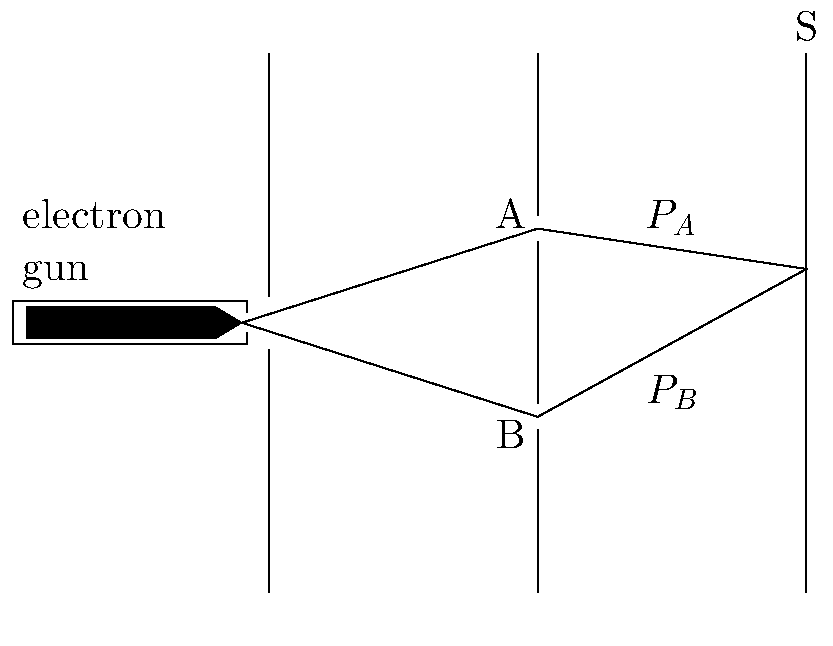
\includegraphics[width=.5\textwidth]{./Figure/Fig2-1.pdf}}
\end{figure}

Next, we generalize this approach as shown in Fig. \ref{Fig2-2}. Different from Fig. \ref{Fig2-1}, there is not just one screening shield, but many, and there are not two slits in each, but a large number (Fig. \ref{Fig2-2}a).

Depending on the way at each screen, many different combinations $c$ for passing through the slits are possible, each corresponding to an amplitude $a_c$, the total amplitude $a$ is given by $\sum _ { c } a _ { c }$. By increasing the number of screening layers and slits more and more, and finally reaching an infinite number, each screening layer will have many slits and finally will disappear. The interval between the gun and the screen will become a continuous space (Fig. \ref{Fig2-2}b), and depending on the “combination of slits” the path will mutate to an arbitrary path from the gun to the screen, and “the sum of all amplitudes of possible ways” will mutate to an integral over the paths, that is, the path integral. That is to say, the principle that “the amplitude corresponding to a transition from a starting point to an end point corresponds to an integral over the amplitudes of all possible paths linking these two points” can be regarded as the principle of quantum mechanics.

\begin{figure}[!b]
\begin{picture}(450,100)
\put(0,5){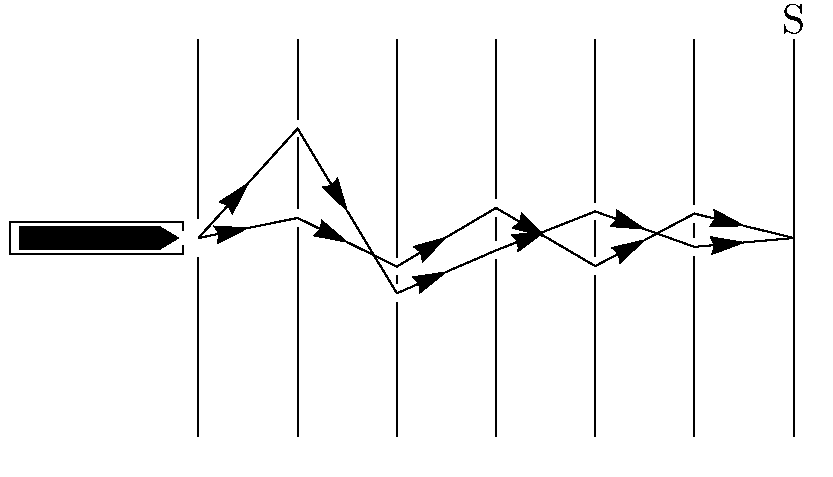
\includegraphics[width=.48\textwidth]{./Figure/Fig2-2a.pdf}}
\put(200,5){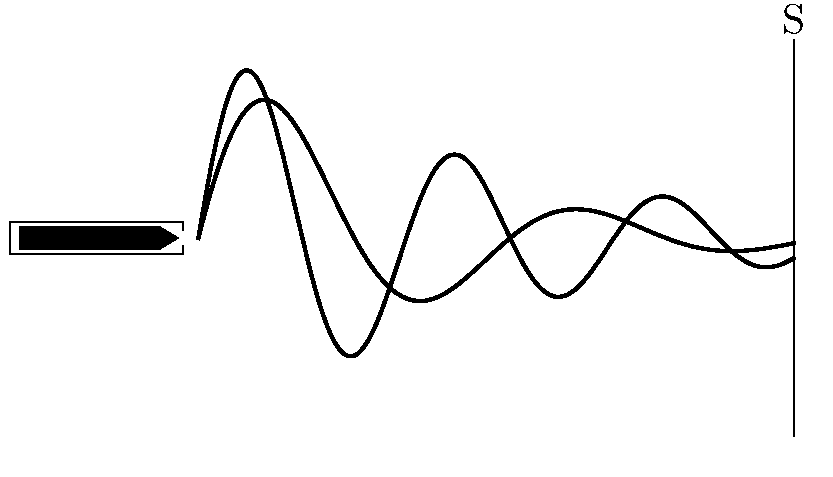
\includegraphics[width=.48\textwidth]{./Figure/Fig2-2b.pdf}}
\put(100,0){(a)}
\put(300,0){(b)}
\end{picture}
\caption{a, b. Generalization of the interference experiment of Fig. \ref{Fig2-1}. The number of screens and the number of slits in the screen is increased. }\label{Fig2-2}
\end{figure}

When considering quantum mechanics, one might have in mind the wave function, and the Schr\"{o}dinger equation of the wave function, all describing wave properties of the particle. It should be possible to link this description with the picture of the path integral described above by using the superposition principle of waves. However, it required the genius of Feynman to make this discovery.


We now turn to exact mathematics. We start from the Schr\"{o}dinger equation 
\be\label{eq2.1.1}
\begin{aligned} \mathrm { i } \hbar \frac { \partial \psi ( x , t ) } { \partial t } & = - \frac { \hbar ^ { 2 } } { 2 m } \frac { \mathrm { d } ^ { 2 } \psi ( x , t ) } { \mathrm { d } x ^ { 2 } } + V ( x ) \psi ( x , t ) \\ & = H \psi ( x , t ) \end{aligned}
\ee
For a moment, we restrict the motion of the particle to a one-dimensional space with space coordinate $x$. 

As shown in \eqref{eq1.1.3}, it is possible to integrate \eqref{eq2.1.1} formally
\be\label{eq2.1.2}
| \psi \left( t ^ { \prime } \right) \rangle = U \left( t ^ { \prime } , t \right) | \psi ( t ) \rangle = \mathrm { e } ^ { - ( 1 / \hbar ) H \left( t ^ { \prime } - t \right) } | \psi ( t ) \rangle
\ee
We choose $t' > t$. Equation \eqref{eq2.1.2} describes the time evolution of the state $| \psi ( t ) \rangle$ occurring at t through during the time $t'-t$, leading to the state $| \psi ( t' ) \rangle$. Not the wave function can be expressed with the path integral mentioned before, but the operator $U \left( t , t ^ { \prime } \right)$ describing the time evolution. In \eqref{eq2.1.2}, the label $x$ has been omitted intentionally, because $| \psi ( t ) \rangle$ should be regarded as a continuous infinite dimensional vector with components $\psi ( x , t )$ labelled by $x$, and $U \left( t ^ { \prime } , t \right)$ should be regarded as a matrix with components $U \left( x ^ { \prime } , t ^ { \prime } ; x , t \right)$. 






























































































